\documentclass{beamer}
\usetheme{Boadilla}
\usepackage{graphicx} % Required for inserting images
\usepackage{amsthm}
\usepackage{amsmath}
\usepackage{amssymb}

\title{Stability Analysis in Dynamical Systems}
\author{Siddharth K}
\date{July 2024}

\newcommand{\dx}{\dot{x}}
\newcommand{\dy}{\dot{y}}
\newcommand{\du}{\dot{u}}
\newcommand{\dth}{\dot{\theta}}
\newcommand{\bx}{\textbf{x}}
\newcommand{\dbx}{\dot{\bx}}
\newcommand{\ddx}{\ddot{x}}
\newcommand{\ddth}{\ddot{\theta}}

\begin{document}

\begin{frame}
    \titlepage
\end{frame}

\begin{frame}{Dynamical Systems}
    Dynamical system: a system that evolves over time.
    \vfill
    Described by:
    $$\dx = f(x(t), t)$$
    where $x \in \mathbb{R}^n$ and $\dx = \frac{dx}{dt}$. \\
    
    \begin{definition}[Fixed Point]
        A \textbf{fixed point} (or equilibrium point), $x^*$, is a state where $f(x^*, t) = 0$.
    \end{definition}
    
\end{frame}

\begin{frame}{Stability}

    Initial condition: $x(0)$. \\
    \pause
    \begin{definition}[Stable]
        A fixed point $x^*$ is stable if for every $\epsilon > 0$ there exists a $\delta > 0$ such that if $\|x(0) - x^*\| < \delta$, then for all $t \ge 0$ we have $\|x(t) - x^*\| < \epsilon$. The fixed point is called unstable otherwise.
    \end{definition}
    \pause
    \begin{definition}[Attracting]
        A fixed point $x^*$ is attracting if there exists $\delta > 0$ such that if $\|x(0) - x^*\| < \delta$ then $$\lim_{t \to \infty} x(t) = x^*.$$
    \end{definition}
    \pause
    \begin{definition}[Asymptotically Stable]
        A fixed point $x^*$ is asymptotically stable if it is stable and attracting.
    \end{definition}
    
\end{frame}

\begin{frame}{Linear Systems}

    Linear System:
    $$\dx = Ax$$
    where $A \in \mathbb{R}^{n \times n}$.
    \vfill
    
    \begin{theorem}
        A fixed point $x^*$ of the linear system $\dx = Ax$ is asymptotically stable if all eigenvalues of $A$ have negative real parts.
    \end{theorem}
    
\end{frame}

\begin{frame}{Linearization}
    Given
    $$\dx = f(x)$$
    define perturbation
    $$u = x - x^*$$
    $$\du = \dx = f(x) = f(x^* + u)$$
    \pause
    Taylor expansion:
    $$\du = f(x^*) + J(x^*)u + \text{higher order terms}$$
    $$\text{higher order terms} \approx 0$$
    $$\du \approx f(x^*) + J(x^*)u = J(x^*)u$$
    $$\dx \approx J(x^*)(x - x^*)$$
    \pause
    If the eigenvalues of $J(x^*)$ are negative then the fixed point $x = x^*$ is asymptotically stable.
        
\end{frame}

\begin{frame}{Control Theory}

    Dynamics of a controlled system:
    $$\dx = f(x, u)$$
    where $x \in \mathbb{R}^n$, $u \in \mathbb{R}^m$.
    \pause
    \vfill
    Linear system with control:
    $$\dx = Ax + Bu$$
    where $A \in \mathbb{R}^{n \times n}$, $B \in \mathbb{R}^{n \times m}$.
    \pause
    \vfill
    Feedback control:
    $$u = -Kx$$
    where $K \in \mathbb{R}^{m \times n}$. So
    $$\dx = Ax - BKx = (A - BK)x.$$
    Choose $K$ such that the eigenvalues of $A - BK$ are negative.
    
\end{frame}

\begin{frame}{Spring-Mass-Damper System}

    \begin{figure}
        \centering
        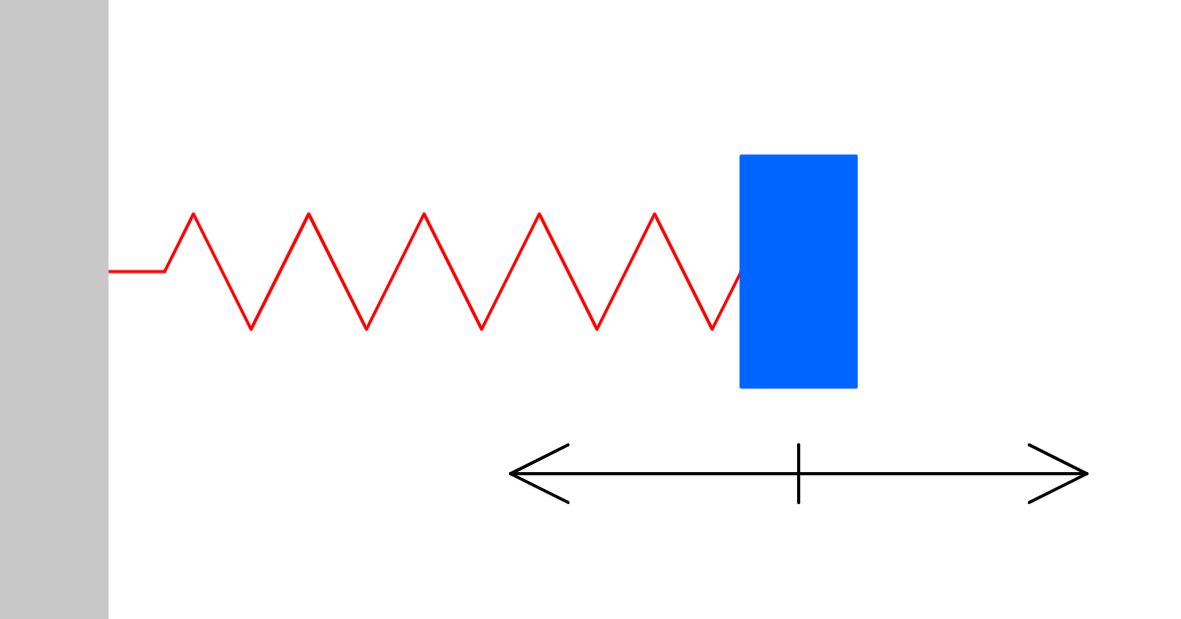
\includegraphics[width=0.4\linewidth]{Spring Mass Damper.png}
        \caption{Spring-Mass-Damper}
        \label{fig:spring-mass}
    \end{figure}

    Spring-mass-damper system:
    $$\dx = Ax + Bu$$
    where
    $$A = 
    \begin{pmatrix}
        0 & 1 \\
        -2 & 3
    \end{pmatrix}, \quad
    B = 
    \begin{pmatrix}
        0 \\ 1
    \end{pmatrix}.$$
\end{frame}

\begin{frame}{Spring-Mass-Damper System (cont.)}

    Let
    $$u = -Kx$$
    where $K = 
    \begin{pmatrix}
        k_1 & k_2
    \end{pmatrix}$. \\
    Evaluating $A - BK$:
    $$A - BK =
    \begin{pmatrix} 0 & 1 \\ -2 & 3 \end{pmatrix} -
    \begin{pmatrix} 0 \\ 1 \end{pmatrix}
    \begin{pmatrix} k_1 & k_2 \end{pmatrix} =
    \begin{pmatrix} 0 & 1 \\ -2 - k_1 & 3 - k_2 \end{pmatrix}.$$
    \pause
    Let eigenvalues be $\lambda$. We have that
    $$\lambda^2 + (k_2 - 3)\lambda + (k_1 + 2) = 0.$$
    \pause
    Arbitrarily choose $\lambda = -2, -5$. They satisfy $$(\lambda + 2)(\lambda + 5) = \lambda^2 + 7\lambda + 10 = 0.$$
    \pause
    $$k_1 + 2 = 10 \implies k_1 = 8,$$
    $$k_2 - 3 = 7 \implies k_2 = 10.$$
    So $K = 
    \begin{pmatrix}
        8 & 10
    \end{pmatrix}$.
    
\end{frame}

\begin{frame}{Nonlinear Dynamics and Control}

    Given
    $$\dx = f(x, u), \quad f(x^*, u^*) = 0,$$
    define perturbations
    $$\Delta x = x - x^*, \quad \Delta u  = u - u^*.$$
    Approximate using Taylor expansion:
    $$\Delta \dx = \dx = f(x, u) \approx f(x^*, u^*) + A\Delta x + B\Delta u,$$
    $$A = \left.\frac{\partial f}{\partial x}\right|_{(x^*, u^*)}, \quad B = \left.\frac{\partial f}{\partial u}\right|_{(x^*, u^*)}$$
    $$\Delta \dx \approx A\Delta x + B\Delta u$$
    
\end{frame}

\begin{frame}{Cart-Pole Problem}

    \begin{columns}
        \column{.4\textwidth}
        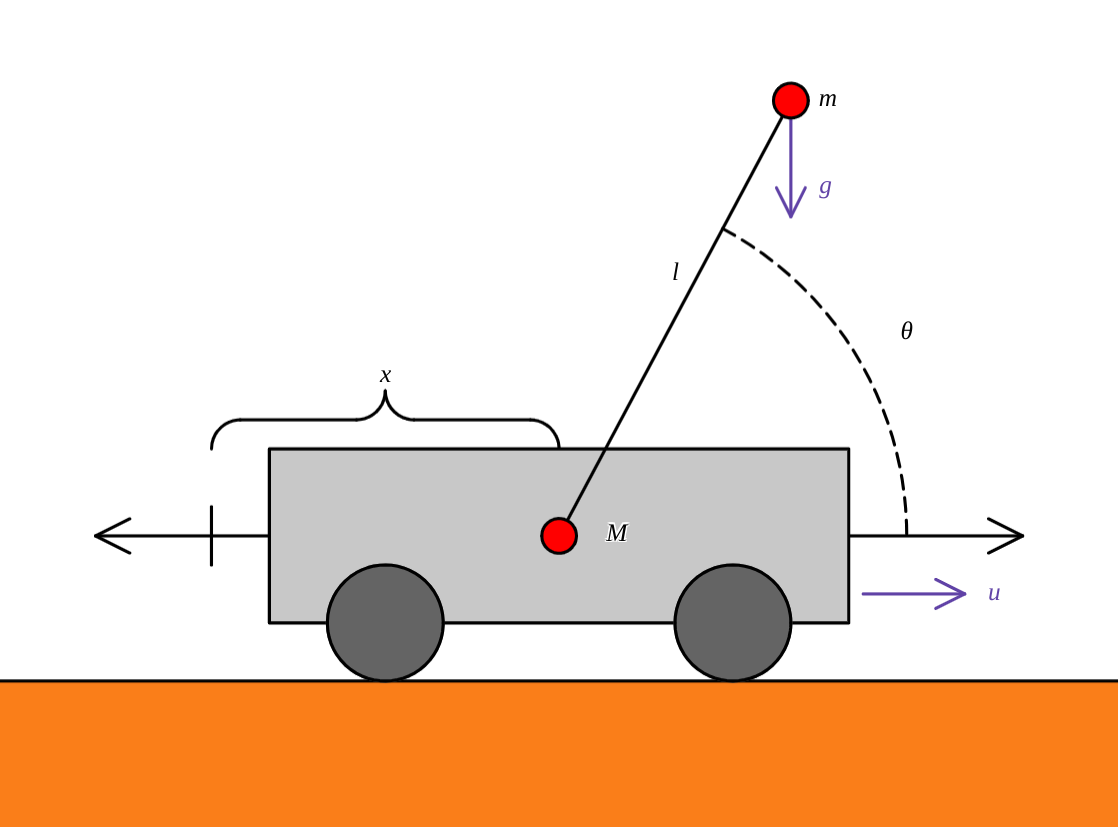
\includegraphics[width=\linewidth]{Cart-Pole Problem.png}
        \column{.6\textwidth}
        Dynamics of the cart-pole problem:
        \begin{align*}
            & (M + m)\ddx + ml\ddth\cos(\theta) - ml\dth^2\sin(\theta) = u \\
            & l\ddth + g\sin(\theta) = \ddx\cos(\theta).
        \end{align*}
        The variables are:
        \begin{itemize}
            \item $x$: Position of the cart
            \item $\theta$: Angle of the pole (upright is $\theta = 0$)
            \item $u: \text{Control force applied to the cart}$
            \item $M: \text{Mass of the cart}$
            \item $m: \text{Mass of the pole}$
            \item $l: \text{Length of the pole}$
            \item $g: \text{Acceleration due to gravity}$
        \end{itemize}
    \end{columns}
    
\end{frame}

\begin{frame}{Cart-Pole Problem (cont.)}

    State vector:
    $$\bx = (x, \dx, \theta, \dth)^T \approx (0, 0, 0, 0)^T.$$
    We can make the approximations
    \begin{align*}
        & \sin(\theta) \approx \theta, \\
        & \cos(\theta) \approx 1, \\
        & \dth^2 \approx 0.
    \end{align*}
    Substituting gives us
    \begin{align*}
        (M + m)\ddx + ml\ddth &\approx u \\
        l\ddth + g\theta &\approx \ddx.
    \end{align*}
    
\end{frame}

\begin{frame}{Cart-Pole Problem (cont.)}

    \begin{align*}
        (M + m)\ddx + ml\ddth &\approx u \\
        l\ddth + g\theta &\approx \ddx.
    \end{align*}
    Linearization gives us
    $$\dbx \approx A\bx + Bu$$
    where $$A = 
    \begin{pmatrix}
        0 & 1 & 0 & 0 \\
        0 & 0 & \frac{mg}{M + 2m} & 0 \\
        0 & 0 & 0 & 1 \\
        0 & 0 & -\frac{Mg + mg}{l(M + 2m)} & 0
    \end{pmatrix}, \quad B = 
    \begin{pmatrix}
        0 \\
        \frac{1}{M + 2m} \\
        0 \\
        \frac{1}{l(M + 2m)}
    \end{pmatrix}.$$
    Let
    $$u = -Kx$$
    and find eigenvalues of $A - BK$ (requires numerical methods).
    
\end{frame}

\begin{frame}{Thank You}
    Thank you for listening!
\end{frame}

\end{document}